%!TEX root = ../report.tex

\begin{document}
    \chapter{State of the Art}
    This chapter will discuss the 3D LiDAR datasets available and classify them based on the type of acquisition.
    Also, we will discuss the existing 3D semantic segmentation models, uncertainty estimation methods and Out Of Distribution (OOD) detection methods available.
    \section{3D LiDAR Datasets}
    %Since the advent of AlexNet \cite{alexnet}, deeplearning has been in the rise. 
    %Deep convolutional neural networks are the desired option for image analysis tasks such as classification, detection and segmentation.
    %These deep convolutional networks are successful especially because of two reasons. 
    %First is the architectures and their paralellisation, allowing them to train millions of images on a GPU.
    %Second reason is the development of huge public benchmark datasets such as Imagenet \cite{imagenet}, Pascal VOC \cite{pascalvoc} and COCO \cite{coco} datasets
    %Although deep convolutional networks are huge success in image analysis tasks, they perform poorly on 3D point cloud data.
    LiDAR is one of the central component in the sensor suite for SLAM system in robotic applications \cite{thrun2006stanley}, \cite{patz2008practical}, \cite{hess20162dSLAM} and autonomous driving \cite{li2016vehicle}.
    3D LiDAR data is preferred because it can provide a replica of the 3D geometry of the world represented in the form of point clouds.
    Because of these rich features and widespread use of LiDAR sensors, tasks such as 3D object detection \cite{zhou2018voxelnet}, \cite{PIXOR} and 3D semantic segmentation \cite{qi2017pointnet++}, \cite{3Dmininet} are becoming more predominant area for research.
    
    In this section, we will discuss the available LiDAR datasets for the 3D semantic segmentation task and classify the datasets based on acquisition methods as in \cite{survey3d}.
    \cite{survey3d} classifies the available public datasets into three classes based on the data acquisition process.
    They are \textit{sequential}, \textit{static} and \textit{synthetic} datasets.
    For a sequential dataset, the data is collected as a sequence of frames where a mechanical LiDAR is mounted on top of an autonomous driving platform as in Figure \ref{fig:seq_data_lyft}.
    Figure~\ref{fig:example_sequential} represents an example point cloud from a sequential dataset.
    \begin{figure}[h!]
        \begin{subfigure}{0.45\textwidth}
            \centering
            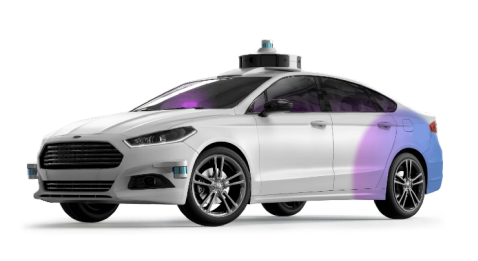
\includegraphics[scale=0.25]{images/sequential_lyft.png}
            \caption{}
            \label{fig:seq_data_lyft}
        \end{subfigure}
        \begin{subfigure}{0.45\textwidth}
            \centering
            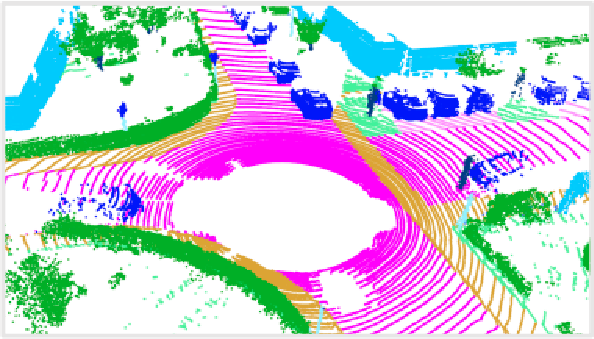
\includegraphics[scale=0.45]{images/SemanticKitti.pdf}
            \caption{}
            \label{fig:example_sequential}
        \end{subfigure}
        \caption{Image (a) depicting the LiDAR mounted on a vehicle to collect sequential data for the Lyft L5 dataset and 
        (b) depicts an example of sequential data from the SemanticKITTI dataset. Images are from \cite{Lyftl5} and \cite{Hu_2020_CVPR_Randla} respectively.}
        
    \end{figure}
    Most of the popular autonomous driving datasets are sequential, but these datasets come with a drawback of sparse points than other datasets.
    
    Static datasets consist of data collected from a stationary viewpoint by a terrestrial laser scanner.
    This kind of dataset captures the static information of the real world, whereas the sequential datasets capture the dynamic movements of the surrounding objects.
    Static datasets find their way into urban planning, augmented reality, and robotics applications. 
    Figure \ref{fig:tls} depicts a terrestrial laser scanner used to capture the static point cloud of an industrial environment, and Figure~\ref{fig:static_scan} represents an example point cloud for a static dataset.
    \begin{figure}[h!]
        \centering
        \begin{subfigure}{0.45\textwidth}
            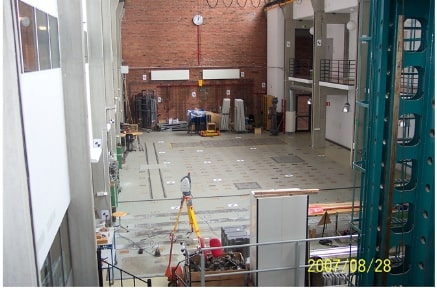
\includegraphics[scale=0.45]{images/TLS.jpg}
            \caption{}
            \label{fig:tls}
        \end{subfigure}
        \begin{subfigure}{0.45\textwidth}
            \centering
            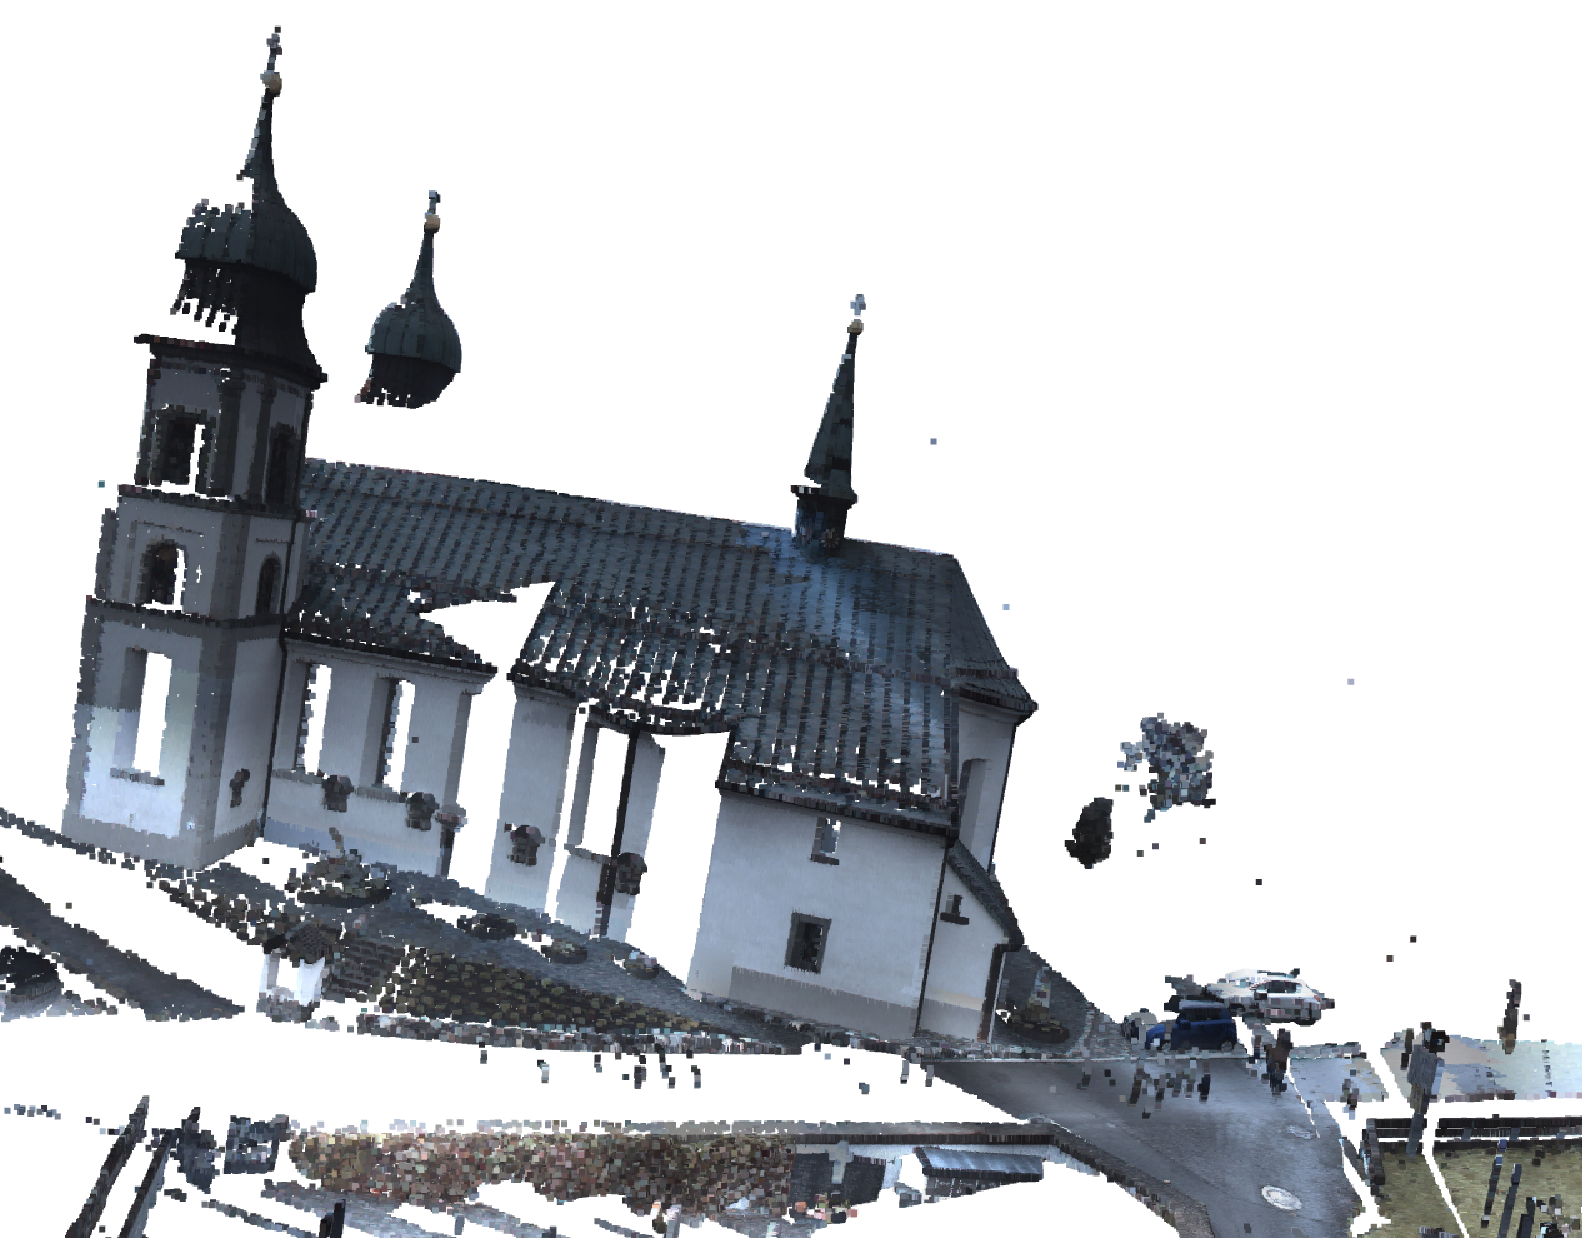
\includegraphics[scale=0.2]{images/sem3d_data/1.pdf}
            \caption{}
            \label{fig:static_scan}
        \end{subfigure}

        \caption{	Image (a) depicting the terrestrial laser scanner in an industrial environment to collect static data with the laser scanner mounted on a yellow tripod in the left corner of the floor and 
        (b) represents the scene of static data from the Semantic3D dataset. The first image is taken from \cite{tls}.}
       
    \end{figure}
    Static datasets are advantageous because they can produce highly dense point clouds leading to rich geometric representations.
    
    The last type of 3D LiDAR dataset is the synthetic dataset. 
    As the name suggests, these datasets are generated from computer simulation. 
    Figure \ref{fig:synthetic} depicts a simulated point cloud in a synthetic dataset called SynthCity.
    Even though synthetic datasets can be generated on a large scale at a cheap cost, they lack the accuracy in detail compared to the point clouds generated from the real world.
    \begin{figure}[h!]
        \centering
        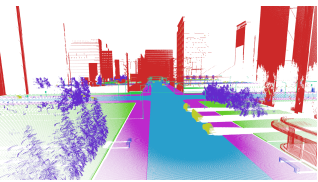
\includegraphics[scale=0.5]{images/synthcity.png}
        \caption{Illustration of a scene in synthetic dataset called SynthCity. Image taken from \cite{griffiths2019synthcity}}
        \label{fig:synthetic}
    \end{figure}
    
    The datasets belonging to the each acquisition type are summed up in  Table \ref{table:3d_lidar_datasets_table}.
    Most of the datasets from Table \ref{table:3d_lidar_datasets_table} are taken from \cite{survey3d} and also as a part of this study, additional new datasets were added to the list.
    The newly added datasets include DALES \cite{varney2020dales}, ScanObjectNN \cite{scanobejctnn} in static acquisition mode and AIO Drive \cite{Weng2020_AIODrive}, Toronto3D \cite{tan2020toronto3d} are additions in the sequential mode.
    % \cite{survey3d} also classifies GTAV \textcolor{red}{\textbf{cite}} dataset as synthetic 3D LiDAR but the corresponding paper doesn't report any LiDAR dataset and proposed only 2D dataset for segmentation.
    The limited number of datasets in 3D LiDAR allowed us to study the characteristics of each dataset, such as each class, data distribution and features of the point cloud. 
    %%%%% It is summarized in Table \textcolor{red}{\textbf{ref}} in Appendix \textcolor{red}{\textbf{chapter number}}
    %%\section{TODO}
    %%\begin{itemize}
    %%     \item[$\bullet$] Explain the table
    %%    \item[$\bullet$] Discuss why SemanticKITTI and Semantic3D are of our interest     
    %%\end{itemize}
    
    \begin{table}[h!]
        %\centering
        \begin{tabular}{c|c|c|c|c|c}%|c}
            \hline
            % acquisition type, dataset, frames, #points, classes, I/O, year
            acquisition mode & dataset & frames & points (in million) & classes & scene type \\  % & pub. year \\
            \hline
            \multirow{7}{*}{static} & Oakland\cite{oakland} & 17 & 1.6 &  44 & outdoor \\ % & 2009 \\ 
                                    & Paris-lille-3D\cite{roynard2018paris} & 3 & 143 & 50 & outdoor \\ % & 2018 \\
                                    & Paris-rue-Madame\cite{paris_rue_madame} & 2 & 20 & 17 & outdoor \\ %& 2014 \\
                                    & S3DIS\cite{Armeni_2016_CVPR_S3DIS} & 5 & 215 & 12 & indoor \\ %& 2016 \\
                                    & ScanObjectNN\cite{scanobejctnn} & - & - & 15 & indoor \\ %& 2019 \\
                                    & Semantic3D\cite{hackel2017semantic3d} & 30 & 4009 & 8 & outdoor \\ %& 2017 \\
                                    & TerraMobilita/IQmulus\cite{TerraMobilita} & 10 & 12 & 15 & outdoor\\ % & 2015 \\
                                    & TUM City Campus\cite{gehrung2017approach_tum_campus} & 631 & 41 & 8 & outdoor\\ % & 2016 \\
                                    & DALES\cite{varney2020dales} & 40 (tiles) & 492 & 8 & outdoor\\ % & 2021\\
            \hline
            \multirow{7}{*}{sequential} & A2D2\cite{geyer2020a2d2} & 41277 & 1238 & 38 & outdoor\\ % & 2020\\
                                        & AIO Drive\cite{Weng2020_AIODrive} & 100& - & 23 & outdoor\\ % & 2020\\
                                        & KITTI-360\cite{Xie_2016_CVPR_KITTI_360} & 100K & 18000 & 19 & outdoor\\ %& 2020\\
                                        & nuScenes-lidarseg\cite{caesar2020nuscenes} & 40000 & 1400 & 32& outdoor\\ % & 2020\\
                                        & PandaSet\cite{PandaSet} & 16000 & 1844 & 37 & outdoor \\ %& 2020\\
                                        & SemanticKITTI\cite{Behley_2019_ICCV} & 43552 & 4549 & 28 & outdoor \\ %& 2019\\
                                        & SemanticPOSS\cite{pan2020semanticposs} & 2988 & 216 & 14 & outdoor \\ %& 2020\\
                                        & Sydney Urban\cite{de2013unsupervised} & 631 & - & 26 & outdoor\\ % & 2013\\
                                        & Toronto-3D\cite{tan2020toronto3d} & 4 & 78.3& 8& outdoor\\ % & 2020\\
    
            \hline
            \multirow{1}{*}{synthetic}  & SynthCity\cite{griffiths2019synthcity} & 75000 & 367.9 & 9 & outdoor \\ %& 2019\\
            \hline
        \end{tabular}
        \caption{3D LiDAR datasets classified based on the acquisition type. Table updated from \cite{survey3d}}
        \label{table:3d_lidar_datasets_table}
    \end{table}
    
    We chose the Semantic3D dataset as the in-distribution (ID) training dataset from the available datasets. 
    S3DIS is chosen as an out-of-distribution (OOD) dataset as S3DIS is much different from Semantic3D.
    Chapter~\ref{ch:benchmark} represents the detailed discussion on datasets and benchmarking.

    \section{3D semantic segmentation models}

    This section will discuss the methods available for 3D semantic segmentation.
    The discussion includes a brief peek into traditional 3D semantic segmentation methods and the study of deep learning methods for 3D point cloud segmentation.

\subsection{Traditional approach}
Traditional methods involve a complex features extraction and passing these features to a classification algorithm such as Support Vector Machines or Random Forests to classify each point in the point cloud.
Various authors developed various methods to extract the features from the input point cloud.
Some of these methods include segmentation from edge information \cite{bhanu1986range}, construction of complex graph pyramids \cite{koster}.
3D Hough transforms as in \cite{vosselman20013d} and application of RANSAC \cite{schnabel2007efficient} and \cite{tarsha2007hough}.
These traditional methods are outdated as DNNs proved to be better at feature extraction.

\subsection{Deep learning approach}
\label{sec:dl_approach}
Deep learning based models are efficient at segmentation and can be divided into three types.
The initial type includes the point-based models where the model directly feeds on the 3D point cloud.
Then the other type includes projection based models where the model takes in projected points into a 2D image, either a range image or a bird's eye view.
The final type of model includes the use of the graph neural networks.

Let us look briefly into the point-based methods. Point-based methods majorly utilize fully connected layers or traditional convolutional layers.
The major revolution in Deep learning based 3D semantic segmentation came after the PointNet proposed in \cite{Qi_2017_CVPR_pointnet}.
Pointnet applied Multi-Layer Perceptrons (MLP) to extract a global feature vector from the unstructured point cloud and then classify it using the fully connected layers.
Since only Pointnet can extract local features, Pointnet++ proposed in \cite{qi2017pointnet++} applies Pointnet over the point cloud iteratively to extract features at a global scale and then classifies.
Even though the performance of Pointnet and Pointnet++ are weak, they served as a backbone for new architectures such as RandLA-Net proposed in \cite{Hu_2020_CVPR_Randla}.
Similar to PointNet, RandLA-Net employs MLP for feature extraction and then these features are passed through attention and then for classification.
 Section~\ref{sec:meth_randla} describes in detailed about RandLA-Net.
It is one of the best-performing models with lower parameters across Static and Sequential datasets.

The other flavours of point-based methods include projection onto a d-dimensional lattice or making the point cloud structured.
SPLATNet \cite{Su_2018_CVPR_splatnet} utilizes the Bilateral Convolutional layers to project data on a d-dimensional lattice and then classify.
Whereas LatticeNet proposed in \cite{rosu2019latticenet} projects the data onto sparse lattice, then classified and learns the reprojection to 3D using a novel DeformSlice module.
Even though SPLATNet and LatticeNet use projection, they are grouped under point-based models because the model learns these projections.
\cite{spvnas} proposed SPVNAS where the point cloud is voxelized, then classified and then devoxelized.
Finally, \cite{Tatarchenko_2018_CVPR_tangconv} proposed Tangent Convolution similar to standard convolutions but with extra multiplications.

Let us first discuss the models that project the data onto a 2D range image in projection-based models.
First, of this kind is SqueezeSeg proposed in \cite{Sequeseseg_2018}. It employs SqueezeNet for 2D segmentation and then reprojected to 3D using Recurrent Conditional Random Fields.
Since the performance of SqueezeSeg is weak, later versions of SqueezeSeg, such as SqueezeSegV2 proposed in \cite{SqueezeSegv2} and SqueezeSegV3 as in \cite{xu2020squeezesegv3} employ Context Aggregation Module and Spatially Adaptive Convolutions respectively to improve performance relative to SqueezeSeg.
RangeNet proposed in \cite{Milioto2019} even has three versions similar to SqueezeSeg, where the first two versions use the DarkNet21 and DarkNet53 model for 2D semantic segmentation and then reproject the data back to 3D.
The final version uses the DarkNet53 model with kNN to reproject the 2D range image to 3D after segmentation.
Similarly 3DMiniNet \cite{3Dmininet} and KPRNet \cite{kochanov2020kprnet} projects data to range image for segmentation with former using MiniNetV2 as backbone model and later using ResNeXt-101 as backbone.

We now discuss the projection-based models, which involve bird eye view projection.
These models are relatively new to the field but have comparable performance to the existing models.
SalsaNet \cite{salsanet2020} and SalsaNext \cite{SalsaNext_2020} are the two models to employ bird eye view projection as input and both uses ResNet model as backbone.
The latter one utilizes Lovasz-Softmax loss along with cross-entropy. SalsaNext also involves the study uncertainty by modelling SalsaNext as a Bayesian Neural Network to the best of our knowledge.
PolarNet \cite{polarnet} and Cylinder3D \cite{zhu2020cylindrical} are recent models to incorporate bird eye view projection into the segmentation pipeline.
The projections, such as 2D range image and bird's eye view projection, are performed prior to model input.

Table \ref{tab:model_relatedwork} illustrates the detailed summary of each model along with the number of parameters.
Finally, graph neural networks \cite{dyn_graph_cnn} are also able to produce better segmentation results. However, this study is limited to standard deep learning models, so this study does not include graph neural networks.

    \section{Uncertainty estimation methods}
    This section will discuss existing methods to estimate uncertainty in deep neural networks.
    Here we divide the uncertainty estimation methods into ensemble methods, Bayesian methods.
    The methods discussed here primarily estimate epistemic uncertainty. Only test time augmentation and gaussian density models estimate aleatoric uncertainty.

    \cite{matias_uncertainty} argues that there are two kinds of uncertainties, they are epistemic and aleatoric uncertainty.
    Epistemic uncertainty is uncertainty in the model becuase of lack of adequate training data or lack of proper model specification.
    \cite{matias_uncertainty} argues that the epistemic uncertainty is most helpful in OOD detection.
    This is because during the training, model parameters trains to a particular distribution of data, and must produce high uncertainty estimates when they observe data from different distrbution.
    Aleatoric uncertainty is irreducible and as it is a property of the data like measurement noise.
    An example of aleatoric uncertainty in point cloud can be incorrect data from the LiDAR scanner collected on a foggy day, as fog reflects most of the laser rays creating disturbances in the scan and also limiting the range.
    \subsection{Ensemble methods}
    Deep ensembles first proposed in  \cite{lakshminarayanan2016simple} is the most prominently used method for uncertainty estimation.
    They exploit the combinatory power of multiple models.
    Multiple instances of the model are initialized randomly, and the same input is fed into all the instances.
    The random initialization leads to slightly different optimization for each model instance. The final output scores from each model are combined by simple averaging.
    Deep ensembles are known to improve the model's overall performance but come with a cost of computational complexity and resource intensiveness.
    Another advantage of using deep ensembled are the lowest correlation between the model instances as the training of the instances are done differently.
    These lower correlation figures lead to the diverse predictions from each model instance.
    In detailed explantion about deep ensembles can be found in Section~\ref{sec:meth_deepensembles}.

    Because of the higher computational complexity and resource intensiveness, there exist multiple flavours of the deep ensembles, such as deep sub-ensembles \cite{deep_subensembles} and masksembles \cite{masksembles}.
    Deep sub-ensembles divide the network into trunk and head.
    The main idea here is to train multiple instances of the head with the same trunk. For example, a trunk can be feature extraction layers in a deep classification network, and the head can be the classification layers.
    Since the primary motivation of the subensembles is to improve the training speed, there is a minute drop in performance compared to deep ensembles as it is a tradeoff between the computational time and quality of uncertainty.
    Masksembles proposed in \cite{masksembles} are relatively new and are a combination of deep ensembles with MC-Dropout.
    Dropout proposed in \cite{Dropout} includes dropping of random neurons. In contrast, with Masksembles, a predefined mask is stated for each layer, and only those specific neurons are dropped every time.

    Other methods include snapshot ensembles \cite{snapshot_ensembles} which iterates over the multiple local optima in the optimization landscape using cyclic learning rate. 
    The model parameters are saved at each of the local optima. 
    All of the other flavours of deep ensembles are proposed to reduce the effect on time, but the memory requirements remain mostly the same except for the subensembles.
    The other problem with snapshot ensembles is that the optimization landscape in deep neural networks is poorly studied, so one cannot say with certainty that the model saved at two local minima is uncorrelated.
    There also exists a neural ensemble search \cite{NAS_Ensembles} where the neural architecture search is applied over the ensembles.
    Instead of using various instances of the same model, authors in \cite{NAS_Ensembles} use various instances of various models in the architecture search space.
    In this thesis, we chose to use deep ensembles because of ease of implementation, and deep ensembles also act as a baseline comparison for other ensembles methods in the future.

    \subsection{Bayesian methods}
    Existing neural networks are trained in maximum likelihood, resulting in point estimates for the weights.
    The main idea behind Bayesian neural networks is to use a distribution over the network parameters.
    Instead of a single fixed weight tensor for a layer in a neural network, a weight tensor is drawn from the distribution for each forward pass.
    The parameters are estimated for input during training by using the Bayes rule and expressed in Equation~\ref{eq:bayes_1}.
    \begin{equation}
        p(\theta|x, y) = \frac{p(y|x, \theta)p(\theta)}{p(y|x)} = \frac{p(y|x, \theta)p(\theta)}{\int p(y|x, \theta) p(\theta) d\theta} \label{eq:bayes_1}
    \end{equation}
    Here $\theta$ represents network parameters (weights), $p(\theta)$ represents prior distribution over $\theta$, and x and y represent the input data. In our case, x represents the input point cloud and y its corresponding semantic point labels.
    During inference, the labels are calculated by Bayesian model averaging as given in below Equation~\ref{eq:bayes_2}.
    \begin{equation}
        p(y_t|x_t, x, y) = \int p(y_t|x_t, \theta)p(\theta|x, y)d\theta \label{eq:bayes_2}  
    \end{equation}
    Here $\theta$ represents trained network parameters, x and y represent the training set, and $x_t$ and $y_t$ represent the test set.
    The integrals in the Equations~\ref{eq:bayes_1} and \ref{eq:bayes_2} cannont be computed because $\theta$ is the continous space and so iterating over all possible values of $\theta$ are not feasible.
    So to achieve tractable $\theta$, there exist various approximation methods such as Variational Inference (VI), Laplace approximation and Monte Carlo sampling.

    VI is an approximation method where the posterior probability $p(\theta|x, y)$ is approximated by specific distributions represented by $q(\theta)$.
    Kullback-Liebler Divergence (KLD) is used as a measure to calculate the difference between the two distributions. 
    Since KLD cannot be optimized directly because of the posterior distribution, a function called Evidence Lower BOund (ELBO) similar to KLD is proposed.
    \cite{Gaussian_Priors} representes the $q(\theta)$ as a gaussian approximation and \cite{weight_uncertainty} proposed bayes by backprop to extend stochastic VI for non gaussian priors.
    \cite{Non_Gaussian_Priors} provides a stochastic variational inference that is ELBO loss over mini-batch of data and also assumed the network parameter priors are to be gaussian.
    \cite{Flipout} makes use of the reparameterization trick for the reduction in variance in gradients. The Reparameterization trick led to the reformulation of ELBO loss which made it compatible with standard backpropagation.

    Another widely known example for VI is Monte Carlo Dropout (MC-Dropout), in which the dropout layers are reformulated as random variables with Bernoulli distribution.
    As in \cite{bhandary2020evaluating}, and \cite{gawlikowski2021survey} that training with dropout layers can be formulated as VI, and predictive uncertainty can be calculated during inference by applying MC-Dropout during inference.
    The other flavour of MC-Dropout is that the random incoming activations to the node are dropped instead of the nodes themselves, and this method is called Monte Carlo Dropconnect (MC-Dropconnect) as proposed in \cite{gawlikowski2021survey}.
    An example of MC-Dropout and MC-Dropconnect is depicted in Figure~\ref{fig:Dropout_Connect}.
    \begin{figure}[htbp]
        \begin{subfigure}{0.33\textwidth}
            \centering
            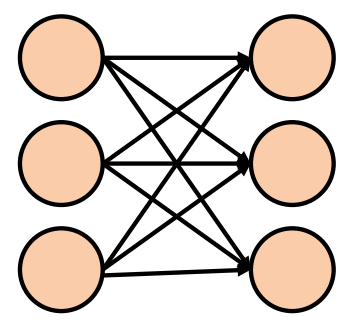
\includegraphics[scale=0.33]{images/BaseNW_SOTA.png}
            \caption{}
        \end{subfigure}
        \begin{subfigure}{0.33\textwidth}
            \centering
            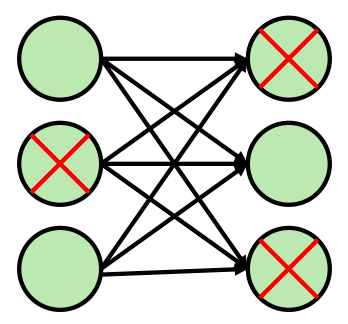
\includegraphics[scale=0.33]{images/Dropout_SOTA.png}
            \caption{}
            \label{fig:SOTA_Dropout}
        \end{subfigure}
        \begin{subfigure}{0.33\textwidth}
            \centering
            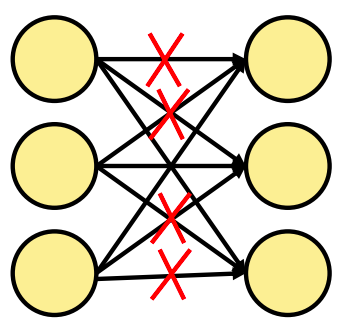
\includegraphics[scale=0.33]{images/DConnect_SOTA.png}
            \caption{}
            \label{fig:SOTA_Dconnect}
        \end{subfigure}
        \caption{Figure (a) depicting the connections of the regular fully connected layers with nodes and connections between them,
        (b) representing the MC-Dropout where few nodes are dropped randomly and 
        (c) representing the MC-Dropconnect where the weight connections are dropped randomly. All the images are taken from \cite{UQ_Survey}.}
        \label{fig:Dropout_Connect}
    \end{figure}
    Another method for estimating uncertinty is flipout as proposed in \cite{Flipout}.
    Although flipout was proposed to decorrelate gradients in a minibatch by sampling independent weight perturbations for each example, it can be used for variational inference and detailed description is provided in Section~\ref{sec:meth_flipout}.
    
    % \textcolor{red}{Need refactoring a bit}
    % Sampling methods also called as Monte Carlo methods (not to be confused to Monte Carlo Dropout or Monte Carlo Dropconnect) estimate uncertainty without any approximation of parametric model.
    % The most popular method in the category of sampling methods is Markov Chain Monte Carlo (MCMC) sampling stated in \cite{Bishop_Book}.
    % Hamiltonian Monte Carlo (HMC) is an another variant of MCMC method and is considered as gold standard algorithm for Bayesian inference as stated in \cite{HMC}.
    % Laplace approximaiton methods make use of second order Tayler series approximation to estimate $p(\theta|x, y)$.
    % Uncertianty in the laplace approximation methods is calculated by taking Hessian matrix of $log(p(\theta|x, y))$ and can be applied to existing trained neural networks as in \cite{Laplace_approx}.
    % Sampling methods and laplace approimation methods arenot studied because the former is computationally expensive and later suffers from infeasibility to compute Hessian matrix for deep neural networks.
    
    
    
    \section{Out-of-distribution (OOD) detection methods}
    This section will discuss the existing OOD detection methods for 2D classification and 2D semantic segmentation tasks.
    To the best of our knowledge, ours is the first work to study OOD detection for the task of 3D semantic segmentation.

    The most widely used benchmarked datasets used for 2D classficiation dataset are CIFAR-10 vs SVHN \cite{liang2017enhancing_ODIN}, CIFAR-10 vs LSUN \cite{hendrycks2016baseline_MSP}, and MNIST vs not-MNIST \cite{hendrycks2016baseline_MSP}. 
    Most of the proposed methods for OOD detection in classification tasks are threshold-based methods which are posthoc methods.
    These methods employ a threshold-based detector and do not see the OOD data during the training.
    The baseline method for threshold-based methods is proposed in \cite{hendrycks2016baseline_MSP}.
    \cite{hendrycks2016baseline_MSP} uses Maximum Softmax Probability (MSP) and argues that in distribution dataset has a higher softmax score, and out of distribution dataset has a lower softmax score and computed as in Equation~\ref{eq:SMSP} where $f_i(x)$ is the output of the neural network.
    Since the softmax scores can be overconfident, \cite{liang2017enhancing_ODIN} proposed Out of DIstribution detector for Neural networks (ODIN), which makes use of calibrated softmax score by addition of temperature constant to softmax scores and computed as in Equation~\ref{eq:SODIN} where $f_i(x)$ is the output of the neural network and $T$ is the temperature constant for calibrated softmax scores.
    In addition to calibrated softmax scores, ODIN also adds noise perturbations to the input making the training adversarial.
    ODIN needs access to the OOD samples because the finetuning of perturbation magnitude is based on these samples.
    \begin{equation}
        S_{MSP}(x) = max_i \frac{exp(f_i(x))}{\sum^{C}_{j=1}exp(f_j(x))}  \label{eq:SMSP}
    \end{equation}
    \begin{equation}
        S_{ODIN}(x) = max_i \frac{exp(f_i(x)/T)}{\sum^{C}_{j=1}exp(f_j(x)/T)}  \label{eq:SODIN}
    \end{equation}
    %\begin{equation}
    %    \begin{cases}
    %        ID if S(x) > \delta_t \\
    %        OOD otherwise
    %    \end{cases}
    %\end{equation}
    \cite{lee2018simple_mahalanobis} has proposed a threshold-based OOD detection method using the Mahalanobis distance as a confidence score.
    The Mahalanobis distance is calculated for every activation map of each layer of the network, and these individual Mahalanobis scores are combined to get a confidence score.
    The Mahalanobis distance is calculated between the activation map and each class distribution represented as multivariate gaussian.
    \cite{Maha_plus_ODIN} proposed the use of Mahalanobis distance and ODIN combined for OOD detection and argues that this combination yields better detection of OOD data.
    \cite{ReAct} proposed Rectified Activations (ReAct) for OOD detection wherein applied to the final layer of the neural network before softmax application, and it suppresses the higher activations to a constant, thereby limiting the effect of noise. 
    ReAct operation is defined in Equation~\ref{eq:react} as
    \begin{equation}
        h^{-}(x) = ReAct(h(x); c) \text{ and } ReAct(x, c) = min(x, c) \label{eq:react}
    \end{equation} 
    where $h(x)$ is final layer activations, $c$ is the constant and $h^{-}(x)$ is ReAct output of $h(x)$.
    The score from this ReAct function is thresholded to detect the OOD data. 
    Recent developments in threshold-based models as proposed in \cite{Energy_OOD_1}, and \cite{Energy_OOD_2} is calculation of energy value based on scalar value from logsumexponential operation over softmax scores.
    These energy scores are expected to be low for the In-Distribution (ID) dataset and vice versa for OOD datasets.

    The OOD data samples have higher uncertainty over ID samples, which allows us to use the uncertainty estimation methods for OOD detection.
    \cite{lakshminarayanan2016simple} proposes the deep ensembles to estimate epistemic uncertainty and utilizes predictive entropy from deep ensembles to classify ID vs OOD datasets.
    Similarly, \cite{JAmersfoot_RBF} proposed the use of radial basis function to calculate the epistemic uncertainty and applied threshold over the epistemic uncertainty to classify OOD data.
    \cite{UOOD_BNN} proposes the use of uncertainty estimated from Bayesian Neural Networks (BNNs) to detect OOD.
    It also argues that the choice of prior weights significantly affects the OOD performance.
    It also argues that the OOD detection performance using BNNs is marginally superior to other methods.
    \cite{Grad_UOOD} proposes the calculation of gradients during the inference and compute uncertainty using the calculated gradients and argues that this approach is also comparably effective for OOD detection.
    \cite{UOOD_RL1}, and \cite{UOOD_RL2} applies uncertainty to detect OOD data samples for the task of Deep Reinforcement Learning.
    
    In recent years, OOD detection for the task of 2D semantic segmentation has been getting into the limelight.
    \cite{pixel_OOD} proposes the adaption of a few above discussed OOD detection methods to the task of 2D semantic segmentation with few or no modifications.
    \cite{pixel_OOD} also proposed benchmarked datasets for OOD detection at pixel level and introduced a novel OOD detection evaluation metric called MaxIoU.
    \cite{SemSeg_Entropy1}, and \cite{SemSeg_Entropy2} proposed the use of entropy values for OOD detection in 2D semantic segmentation task.
    \cite{MetaSeg} proposed a small fully connected neural network called \textit{MetaSeg} with inputs being the metrics such as entropy, probability margin, meanIoU and variation ratio to classify ID and OOD samples.
    \cite{uncertianty_distillation} proposed uncertainty distillation to compute uncertainty estimates similar to knowledge distillation and argues these uncertainty estimates can be efficiently used for OOD detection.

    

\end{document}
